\chapter{Introduzione}

Negli ultimi anni i dispositivi indossabili per la registrazione di video in prima persona hanno conosciuto una diffusione sempre più ampia. Strumenti come \emph{smart glasses}, \emph{body cameras}, \emph{action cameras} hanno reso possibile la cattura di flussi video continui dal punto di vista dell'utilizzatore, dando origine a quello che viene comunemente definito come \emph{egocentric video}. Ciò che li rende peculiari è la loro capacità di catturare dettagli e prospettive uniche, fornendo una visione diretta dell'attività di chi li indossa.

\begin{figure}[ht]
    \centering
    \begin{minipage}{0.3\linewidth}
        \centering
        \includegraphics[width=\linewidth]{Images/meta_glass.png}\\
        Smart glasses
    \end{minipage}
    \hfill
    \begin{minipage}{0.3\linewidth}
        \centering
        \includegraphics[width=\linewidth]{Images/gopro.png}\\
        Action camera
    \end{minipage}
    \hfill
    \begin{minipage}{0.3\linewidth}
        \centering
        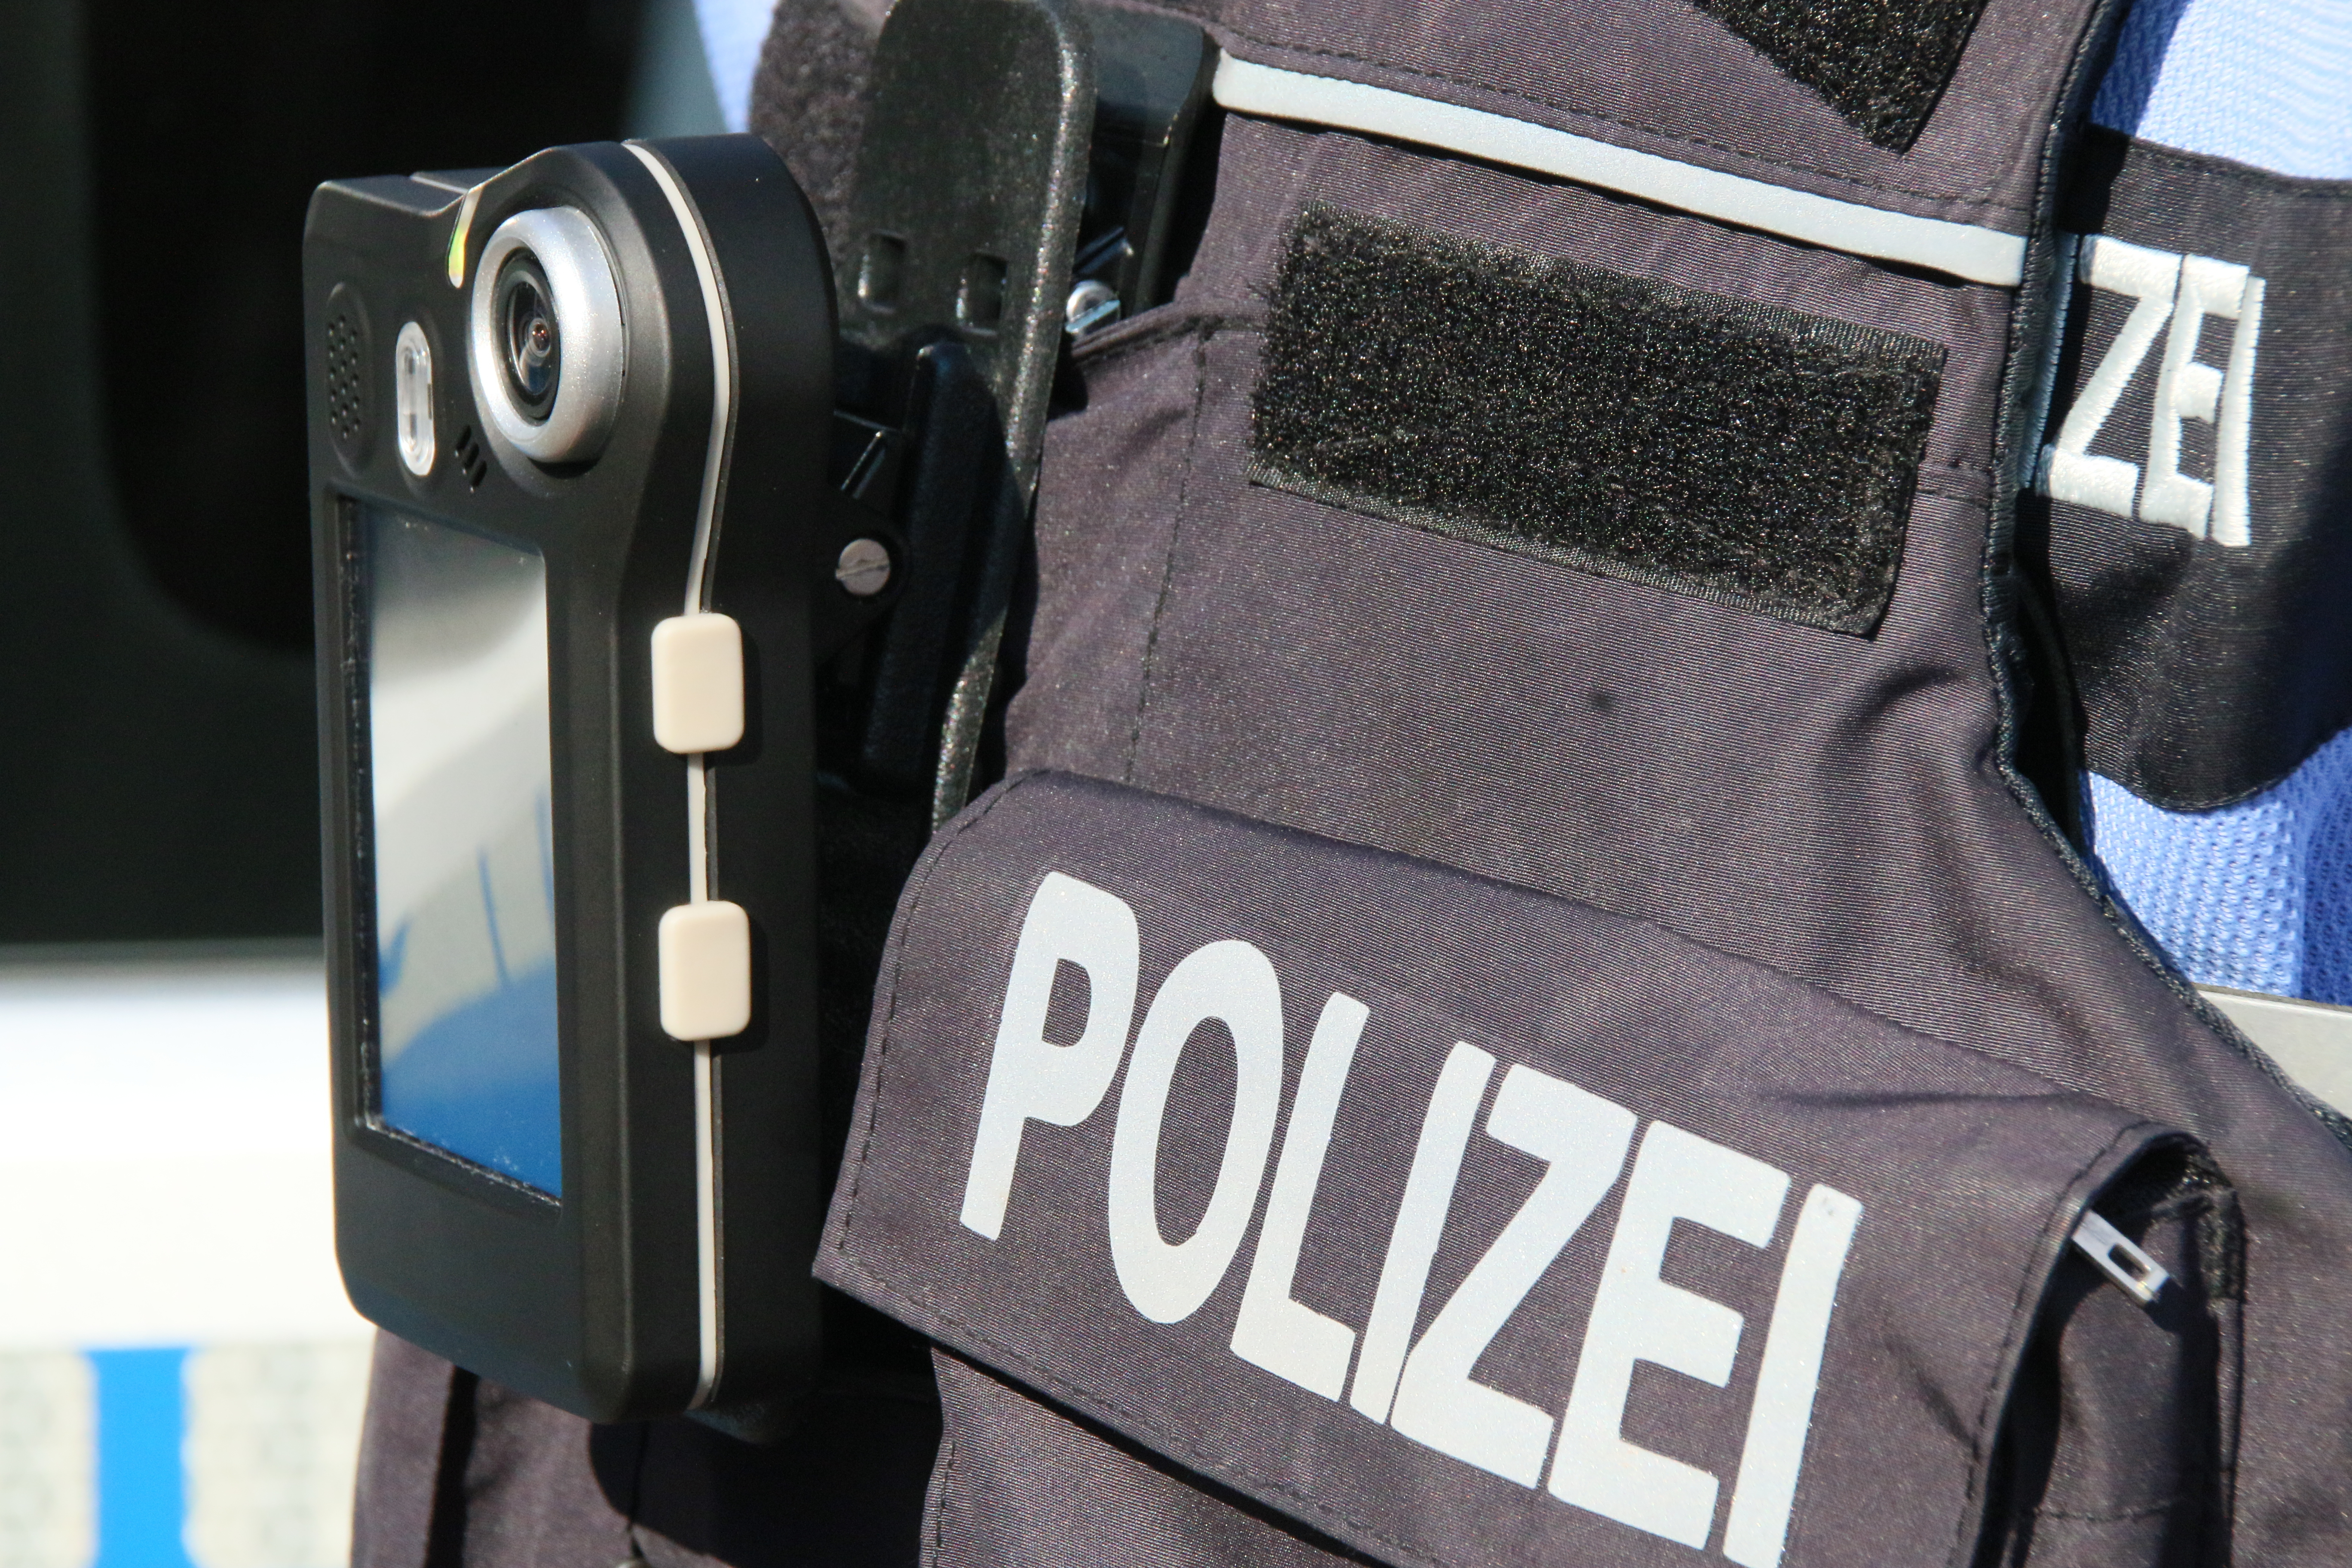
\includegraphics[width=\linewidth]{Images/bodycamera.png}\\
        Body camera
    \end{minipage}
    \caption{Esempi di dispositivi indossabili per la cattura di video egocentrici}
    \label{fig:dispositivi_egocentrici}
\end{figure}

L'adozione crescente di tali dispositivi è stata favorita dalla loro versatilità: da un lato vengono utilizzati per scopi ricreativi e per la condivisione di esperienze personali, dall'altro trovano applicazione in contesti professionali e industriali, dove consentono di documentare procedure complesse e migliorare i processi di formazione e supervisione.

Il principale ostacolo all'analisi di questi contenuti risiede nella loro natura non strutturata. I video in prima persona possono essere considerati come veri e propri flussi di coscienza visivi: lunghi, frammentati, privi di un'organizzazione narrativa chiara e difficili da interpretare. La presenza di movimenti rapidi della fotocamera, variazioni di illuminazione e interazioni simultanee con più oggetti rende complicata l'estrazione di significato. Un'annotazione manuale completa non è praticabile, sia per la mole di dati prodotta sia per la complessità dei contenuti.

Da questa problematica emerge la necessità di costruire una “memoria artificiale” in grado di trasformare i video egocentrici in una rappresentazione più organizzata e interpretabile. In questa tesi analizzeremo innanzitutto i principali contributi presenti in letteratura, per poi concentrarci su \textsc{AMEGO}\cite{goletto2024amego}, un sistema sviluppato per strutturare e rendere interrogabili i video egocentrici e attualmente considerato stato dell'arte nel suo ambito \cite{goletto2024amego}.

Durante la fase sperimentale, valuteremo \textsc{AMEGO} in un contesto diverso da quello in cui era stato testato. Nel lavoro originale è stato valutato sul dataset \emph{EPIC KITCHENS} \cite{Damen2021PAMI}, costituito da video ambientati in cucine domestiche. In questa tesi, invece, l'analisi si concentra sul dataset \emph{ENIGMA-51} \cite{ragusa2023enigma51}, acquisito in contesti industriali, in cui diversi operatori hanno seguito procedure guidate per eseguire attività di riparazione di quadri elettrici. La differenza tra i due domini rende lo studio particolarmente interessante, in quanto consente di valutare la capacità di AMEGO di generalizzare a contesti applicativi mai visti.

In ambito industriale, l'analisi dei video egocentrici è fondamentale per ottimizzare vari aspetti operativi. Garantire ad esempio che le operazioni vengano eseguite nell'ordine corretto migliora i flussi produttivi e riduce il rischio di errori umani. Inoltre, la capacità di riconoscere quali strumenti vengono utilizzati contemporaneamente ad altri oggetti, soprattutto se potenzialmente pericolosi, contribuisce a migliorare la sicurezza dei lavoratori. Quest'ultimo tema prende il nome di \textbf{concurrency}. Sarà di centrale importanza nella fase sperimentale.